\documentclass{article}
\usepackage[german]{babel}
\usepackage{cite}
\usepackage{url}
\usepackage{graphicx}

\author{Phillip Eckstein}
\title{Java Profiling}

\addto\captionsgerman{%
  \renewcommand{\contentsname}%
    {Inhalt}%
}


\begin{document}
    
\selectlanguage{german}
\maketitle
\tableofcontents

\pagebreak

\section{Einleitung}
Diese Arbeit beschäftigt sich mit dem Thema des Profilings in Java. Am Beispiel des Zuul Projektes wird der gesamte Vorgang des Profilings beschrieben. Dabei wird auf alle Wichtigen Aspekte der Auswahl und der Durchführung eingegangen. Als zu profilendes Projekt wird auf die Zuul Anwendung, welche im Modul Objektorientierte Softwareentwicklung der Westsächsisch Hochschule Zwickau erstellt wird zurückgegriffen. Dabei handelt es sich um ein Adventure Spiel mit Grafischer Benutzeroberfläche. Um eine Optimale Auswahl des Profilers zu gewährleisten, wird zuerst eine Anforderungsanalyse durchgeführt. Diese soll hervorheben welche Aspekte des Profilers für diese Arbeit von Bedeutung sind und welche ignoriert werden können. Die Profiler Auswahl soll einen Überblick geben, über die wichtigsten Java Profiler am Markt. Es wird auch darauf eingegangen warum welche Profiler unter Berücksichtigung der vorher in der Anforderungsanalyse aufgestellten Anforderungen geeignet sind und welche nicht. Danach wird das Profiling durchgeführt und dokumentiert. Dabei wird jeder Arbeitsschritt beschrieben und die Ergebnisse festgehalten. Zuletzt wird anschließend eine Auswertung der Ergebnisse durchgeführt, um zu demonstrieren was man durch Profiling herausfinden kann.


\section{Begriffserklaerung}

Im Folgenden wird kurz auf eventuell unklare Begriffe eingegangen. Zunächst soll genauer definiert werden um was genau es sich bei Profilingh handelt. Als Profiling wird eine Tätigkeit beschrieben, bei der mit Hilfe von Programmen und Hilfsmitteln der Bytecode eines Programms, während er Ausführung überwacht wird. Dadurch lässt sich zum Beispiel der Speicherverbrauch und die Laufzeit der einzelnen Befehle besser ermitteln. Die dabei gewonnenen Erkenntnisse sollen danach benutzt werden, um das Programm zu verbessern. Weiter für das Verständnis erforderlich sind folgende Begriffe:
IDE: Integraded Development Enviroment bezeichnet einen Texteditor mit integrierten Tools zum Komplizieren und Ausführen von Code.
Code: Nachfolgend wird der Programmtext der Anwendung auch als Code bezeichnet



\section{Anforderungsanalyse}
Ein Profiler muss Anforderungen erfüllen. Diese ergeben sich abhängig von verschiedenen Einflüssen. Dazu zählen sowohl äußere Einflüsse als auch innere. Als äußere Einflüsse seien Einflüsse anzunehmen, die nicht geändert werden können. Ein Beispiel dafür sind Unternehmensrichtlinien. Als interne Einflüsse sind Kriterien wie die Art, Programmiersprache und Architektur der zu profilenden Software sowie die benutzte IDE. Des Weiteren sollte schon im Voraus geklärt werden welche Teile der Anwendung genauer betrachtet werden sollen. Dies ist wichtig, da verschiedene Profiler wie nachfolgend beschrieben bestimmte Aspekte des Programms besser Testen können. An diese Stelle sei zu erwähnen, dass es wahrscheinlich nicht den einen Besten Profiler für das Projekt gibt, da die meisten Profiler in einem bestimmten Bereich besondere stärken haben. 


Im Rahmen dieser Arbeit soll eine Java Anwendung einem Profiling unterzogen werden. Als IDE kommt Intelij Ultimate von JetBrains zum Einsatz. Daraus ergibt sich bereits die erste Anforderung: Es wird zwingend ein Profiler benötigt, der Java versteht. Eine weitere Anforderung könnte sein, dass das Tool eine möglichst einfache Integration und Bedienung bietet, um unerfahreneren Anwendern das Arbeiten zu erleichtern. Da keine Server Applikation getestet werden soll werden Features wie Online-/ oder Fern-Profiling nicht benötigt. Auch enthält das Projekt keine Datenbank, welche man profilen könnte. Somit sind auch solche Funktionen für den Zweck dieser Arbeit nicht relevant. Eine Integration in die IDE kann jedoch von Vorteil sein, da so die Hürde genommen wird erst ein extra Programm zu starten und Profiling parallel zum Debugging durchgeführt werden kann. Dies führt dazu, dass mehr Bugs im code gefunden werden können. Die zu Profilende Anwendung hat eine Besonderheit: und zwar kann das Spiel sowohl in der Kommandozeile als auch mit einem GUI ausgeführt werden.
Das lässt einen anschaulichen Vergleich zwischen beiden Versionen zu. Eine Funktion, welche bei solch einem Vergleich von Vorteil sein könnte, ist das Erstellen von Abbildungen oder eine andere Form, die Ergebnisse speichern zu können und sie später vergleichen zu können.
Aber selbst der Beste Profiler nützt wenig, wenn man die Ergebnisse nicht sieht. Es ist also wichtig, dass Man schnell und auf einen Blick sieht, was vor sich geht.



\section{Profiler-Auswahl}

Fuer das Profiling von Java stehen eine Vielzahl von Profilern zur Verfuegung. ~\cite{Website:1} Diese werden nachfolgend genauer betrachtet und eine Auswahl auf Basis der in der Anforderungsanalyse betrachteten Kriterien getroffen.
Auf Grund der vielen verschiedenen Profiler kann leider kein Anspruch auf vollstaendigkeit gestellt werden, da auch immer wieder neue auf den Markt kommen. Zur auswahlt stehen sowohl kostenfreie  als auch kostenpflichtige Optionen. Einige der Profiler sind bestandteil anderer Anwendungen wie IDEs, wenn dies der fall wird asuschliesslich der fuer den Profiler relevante Teil betrachtet. Nachfolgend eine kurze Vorstellung der Profiler sowie ein Tablellarischer Vergleich. \ref{tab:1}

\paragraph{JProfiler}

  soll Als erstes betrachtet werden. Bei diesem Tool handelt es sich um eine eigenstaendige Applikation, welche von ej technologies entwickelt wird ~\cite{WEBSITE:2} Sie gilt als eine der am hauefigsten benutzen Profiler fuer Java. ~\cite{WEBSITE:3} JProfiler bietet die moeglichkeit Snapshots, also momentaufnamen aller aktuellen Profiling daten zu erstellen und zu speichern. Ausserdem bietet es vierschiedene moeglichkeiten aufnahmen des gleichen programms zu vergleichen.

\paragraph{YourKit}
 ist ebendfalls eine eigenstaendige Anwendung. Sie wird von der gleichnamigen YourKit GmbH entwickelt ~\cite{WEBSITE:4} YourKit Bietet die moeglichkeit sowohl .NET als auch Java Anwendungen zu Profilen. Es unterstuetzt sowohl lokales als auch remote Profiling und bietet eine gute Integration in Intellij sowie andere IDEs. Des weiteren gibt es die moeglichkeit Snapshots, also momentaufnahmen des Arbeitsspeichers und der CPU Prozesse zu erstellen und mit anderen zu vergleichen.

\paragraph{Java VisualVM}

ist ein Tool, welches einige zeit zusammen mit Oracle Java ausgeliefert wurde. ~\cite{WEBSITE:5} Aktuell wird es ebenfals als eigenstaendige Anwendung vertrieben. Es unterstuetzt alle grundlegenden Methoden des Profilings. Eine Besonderheit ist, das man es ueber Plungins erweitern kann. Das ermoeglicht es, fuer die eigene software massgeschneiderte Profiler zu integrieren.  

\paragraph{Tabellarischer Vergleich}

Nachfolgend der Tabellarische Vergleich zwischen den drei Profilern. 
\begin{table}[h]
  \centering
  \caption{Vergleich von Java Profilern}
  \begin{tabular}{cccc}
    Kriterium & JProfiler & YourKit & Java VisualVM\\
    \hline
    Java Kompatibel & Ja& Ja & Ja\\
    Lokales Profiling &Ja&Ja&Ja\\
    Remote Profiling&Ja&Ja&Ja\\
    Intellij Integration&Ja&Ja&Ja\\
    Speicherprofiling&ja&ja&ja\\
    Prozessprofiling&ja&ja&ja\\
    Snapshot Vergleich&ja&ja&nein\\
    Gute visuelle Darstellung &ja&nein&nein\\
    Erweiterbarkeit&nein&nein&Ja
  \end{tabular}
  \label{tab:1}
\end{table}

\paragraph{Auswahl}
Nach Auswertung der Erkenntnisse ueber die einzelnen Profiler wurde sich fuer Java VisualVM entschieden.  Grund dafuer waren neben den Kosten vor allem das einfach zu verstehende UI sowie die Einfachheit der Anwendung. Da die einfach zu verstehende UI aber ein doch recht subjektives Kriterium ist sei an dieser stelle einmal angemerkt, dass fuer den zweck  dieser Arbeit die meisten Profiler alle anforderungen mehr als ausreichend erfuellen. Die unterschieder liegen hier wie so oft im Detail. 

\section{Durchfuehrung}
Las erstes muss VisualVM herrintergeladen und installiert werden. Den Download link kann man unter Downloads auf Der Hauptseite von VisualVM finden. Nachdem der Zip komprimierte Ordner herruntergeladen wurde muss dieser noch enpackt werden und an eine passende stelle im Nutzerverzeichniss verschoben werden. Da zur Entwicklung der Software Intellij benutzt wird soll der Profiler als naechstes in dieses Integriert werden. Dazu ist es noetig das Plugin VisualVM Launcher von VojTech Krasa zu installieren. Dieses Plugin fuegt Buttons zum Starten des Profiling-Vorgangs mit VisualVM hinzu. ~\cite{fig:Intellij_VisualVM_Button}
\begin{figure}[t]
  \centering
  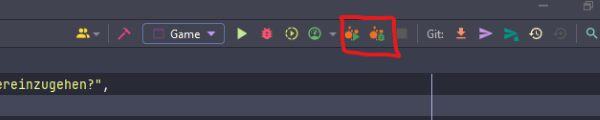
\includegraphics{Intellij_VisualVM_Button}
  \caption{Die neuen Profiling Buttons in Intellij}
  \label{fig:Intellij_VisualVM_Button}
\end{figure}
Bei ersten Starten ist es notwending den Pfad zu der gerade entpackten, ausfuerbaren Datei von VisualVM anzugeben. diese befindet sich normalerweise im gerade entpackten verzeichniss unter /bin. Um das Profiling der Anwendung zu starten reicht es also aus anstelle des ausfueren buttons den Profiler button zu druecken. Nachdem Der profiler gestartet ist wird man von der Startseite begruesst. ~\cite{fig:VisualVM_MainPage} Von hier aus kann man sich anzeigen lassen wieviel last das Programm auf der CPU verursacht, wieviel speicher verbraucht wird und welche methoden ausgefuert werden. Der Overview Tap liefert allegemeine Informationen wie die PID, Wo das programm ausgefuert wird, wie die hauptclasse heist und welche Java 
VM benutz wird. Der Monitor Tab Liefert aaaktuelle daten in grafisch aufbereiteter form ueber CPU last, Heap groesse, geladene klassen und aktive Threads.
Der Threads tab gibt eine Timeline mit allen zu einem bestimmten Zeitpunkt ausgefuerten Threads. Diese sind farblich kodiert um die verschiedenen Zustaende anzuzeigen. Ausserdem sind Die laufzeit und die Gesammtzeit die jeder thread aktiv war zu sehen. Der Letzte Tab enthaelt die Sampling funktionen. Diese ermoeglichen es Aufnahmen von CPU und Speicher zu erstellen um diese spaeter auswerden zu koennen. Diese aufnahmen sind das eigentliche Profiling. VisualVM bietet hier zwei Moeglichkeiten. die Erste ist das Samplen der CPU. Dabei wird der Callstack des Programms sowie sie Ausfuerzeit der einzelnen Threads aufgezeinet. Man kann dabei sowohl Momentaufnamen taetigen als auch das ganze nach beenden als Datei speichern. Auenlich funktioniert das Memory profiling. Hier wird statessen aber aufgezeichnet welche objeckte wieviel Speicher verbrauchen. Nachden nun alle grundfunktionen erklaert sind kommen wir zum interesanten teil, des profilings der eigentlichen Anwendung.

\paragraph{Komandozeilenanwendung}
Als erstes soll die Konsoles version des Spiels geprofiled werden. Dies geschiet indem die main-Methode der Klasse Game ausgefuert wird. Nachdem das Programm gestartet ist wird der Monitor tab geoeffnet. Das Programm wird vorerst ohne eingabe, sozusagen im idle laufen gelassen und es wird beobachtet wie sich die graphen verhalten. Es ist zu beobachten das sich die Applikation langsam aber staetig mehr Speicher einverleibt. So betrauegt der Speicherbedarf der applikation zum start 6,385 MB. Nach 2 Minuten im Idle zustand betrug der Speicherbedarf im test 21,065MB. Der speicherbedarf stieg solange an bis manuell ueber VisualVM die Garbage Collection betaetigt wurde. Dies reduzierte sowohl die maximale Heap Groesse als auch die genutzte Groesse. danach aenderte sich auch das verhalten im idle. So stieg der speicher bedarf nicht erneut auf ueber 30MB sundern wurde nach ca 5 minuten wieder Weniger. CPU last, Klassen und Threads waren hingegen uninteressant. Hier lies sich kein interessantes Verhalten beobachten.
Anschiesssend wurde das spiel ueber die kommandozeile einmal durchgespielt, einmal mit CPU sampling und einmal mit Speichersampling. Beide Ergebnisse wurden gespeichert um sie mit der Grafischen Oberflaeche zu vergleichen.

\paragraph{GUI Anwendung}
Als zweites wurde dei Grafische benutzeroberflaeche Geprofiled. Vorgegangen wurde dabei genauso wie bei der Komandozeile um die ergebnisse Vergleichbar zu halten. Auch hier konnte man direkt einen Speicherbedarfszuwachs erkennen. Allerdings fiel der Speicherbedarf nach ca 7 minuten von allein schlagartig um danach wieder anzusteigen. Nach einiger Zeit Begann der Speicherverbrauch Schlagartig rapide zu steigen und viel in kuerzeren Zeitfrequenzen wieder Schlagartig. Die Applikation startete mit einem Speicherverbrauch von 25,478MB und stieg ueber eine zeit von ca 6 minuten auf  82.108MB an. Danach fiel sie schlagartig auf 22,365MB. Im weiteren verlauf von 2 minuten stieg der Speicherbedarf wieder leicht, nur um dann rapide innerhalb 30 sekunden von ca 39MB auf 116,373MB anzusteigen. Ueber die naechsten 8 minuten wiederholten sich diese Spitzen mit zunehmender Amplitude uns Sinkender frequenz immer weiter. Auch die CPU last zeigte unterschiede. Ungefaer zum selben zeitpunkt, an den die Speicherspitzen auftraten kann man erkennen das die CPU aktivitaet zugenommen hat. Diese war zwar immernoch sehr gering aber erkennbar. Der spitzenwert betraegt in diesem test 3,2\% CPU Last. Anschiesssend wurde das Spiel ueber das GUI einmal durchgespielt, einmal mit CPU sampling und einmal mit Speichersampling. Beide Ergebnisse wurden ebenfalls gespeichert.

\section{Auswertung und Fazit}
\paragraph{Auswertung}
Als erstes wird der Idle Test ausgewertet. Das verhalten beider Versionen der Zuul Applikation ist sehr unterschiedlich. Neben dem erwartet hoehren Speicherverbrauch der GUI legt diese ein gaenzlich anderes Verhalten an den Tag. Aufgrund Der GUI ist ein hoeherer Speicherverbrauch zu erwarten, da mehr Daten geladen werden muessen. Die Aufgenommenen Samples Des Ausführungstests geben aufschluss ueber die Ausführungszeit der einzelnen Methoden. Dabei ist aber kaum ein Unterschied zwischen GUI und Kommandozeile zu erkennen, was daran liegt das meist die Exakt selben Methoden ausgefuert werden. lediglich die methoden fuer die eingabe sind andere. Hier faellt die InitializeFight Methode auf, welche in Kommandozeilenanwendung mit 15ms eine erheblich laengere ausfuerdauer hat. Dies ist aber damit zu erklaeren das in dieser Methode der Parsermodus geweckselt wird um die Kampfkomandos parsen zu koennen, was im GUI umgangen werden kann.

\paragraph{Fazit}
Profiling ist ein gutes Hilfsmittel um Perfomance problemen auf die spur zu kommen. In Java ist es dank einer vielzahl an tools fuer viele verschiedene Anwendungszwecke leicht zu realisieren. Es gibt ausschluss ueber die Laufzeit und den speicherbedarf der Anwendung. So kann man analysieren welche methoden besonders lang benoetigen oder ob es eventuell speicherlecks gibt.

\bibliography{Quellen}
\bibliographystyle{abbrv} 

\pagebreak
\section{Abbildungen}
\begin{figure}[h]
  \centering
  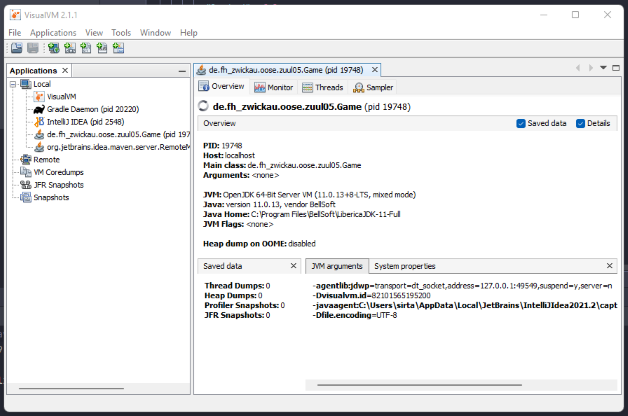
\includegraphics{VisualVM_StartPage.png}
  \caption{Hauptansicht von VisualVM}
  \label{fig:VisualVM_MainPage}
\end{figure}

\begin{figure}
  \centering
  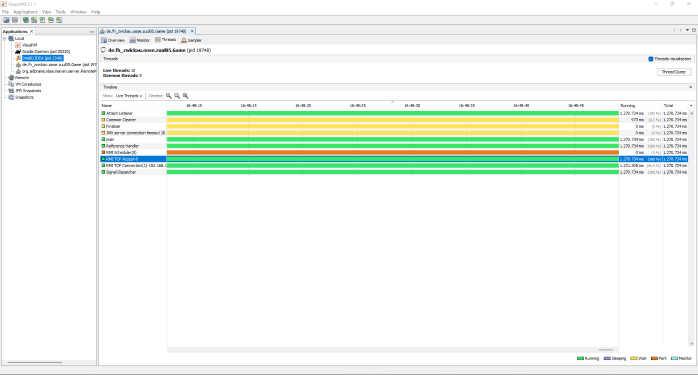
\includegraphics{VisualVM_Threads.png}
  \caption{Thread Ansicht von VisualVM}
  \label{fig:VisualVM_Threads}
\end{figure}

\begin{figure}
  \centering
  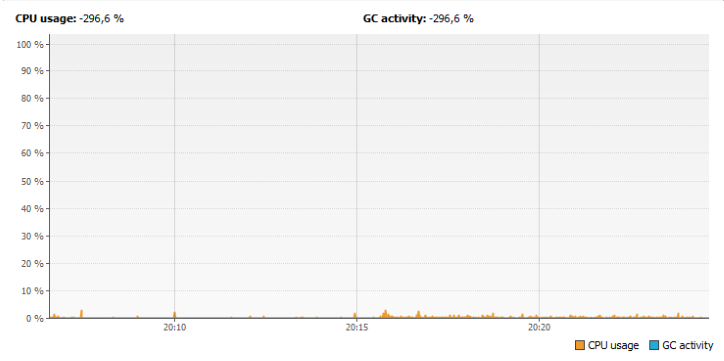
\includegraphics{GUI_CPU_idle.png}
  \caption{CPU auslastung der GUI im Idle zustand}
  \label{fig:GUI_CPU_idle}
\end{figure}

\begin{figure}
  \centering
  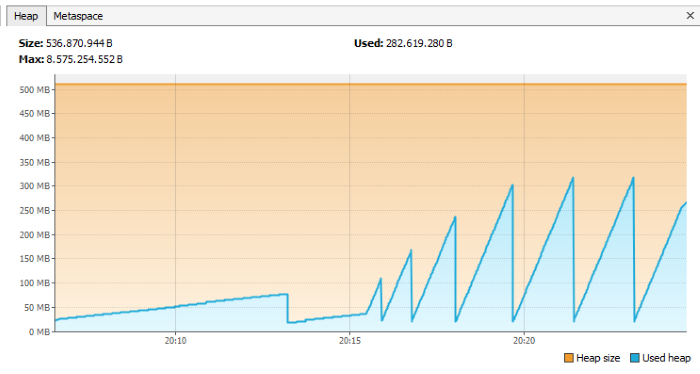
\includegraphics{GUI_Idle.png}
  \caption{Speicherbedarf auslastung der GUI im Idle zustand}
  \label{fig:GUI_MEM_idle}
\end{figure}

\begin{figure}
  \centering
  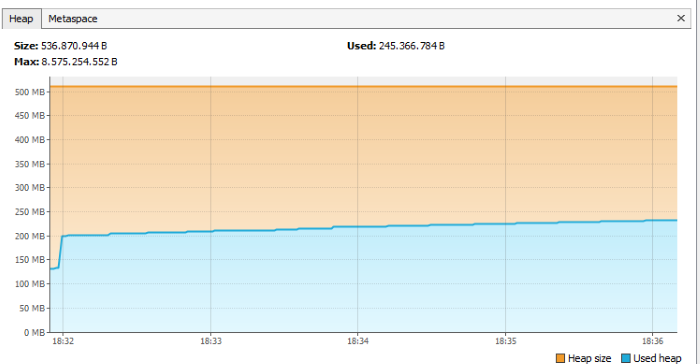
\includegraphics{Memory_console_execute.png}
  \caption{Speicherbedarf der Konsole waerend des Spieldurchgangs}
  \label{fig:Console_mem_Execute}
\end{figure}
\end{document}
